Pour comprendre le manuscrit dans son intégralité, il sera nécessaire de comprendre quelques outils.
Ces outils n'entrant pas dans le récis de la thèse, j'ai choisi de les décrire dans cette section de prérequis.
Premiérement, nous allons décrire le format de représentation moléculaire que nous allons utiliser tout au long du manuscrit, puis nous expliquerons ensuite l'outil mathématique que sont les graphes.

\section{Chimie et SMILES}

\subsection{Représentation 2D de molécules}

\begin{figure}[h!]
  \begin{center}
    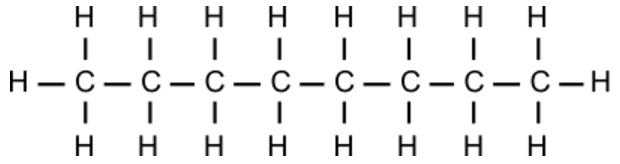
\includegraphics[width=350px]{Figures/bio/Prerequis/developpee.png}
    \caption{\label{dev}Formule développée de la molécule d'octane.}
  \end{center}
\end{figure}

L'ensemble du manuscrit va parler de molécules issues de constructions biologiques.
Une molécule peut classiquement être représentée en 2D sous la forme d'un dessin d'atomes représentés par des lettres, liées par des traits représentant les liaisons covalentes entre atomes (voir figure \ref{dev}).
Cette représentation est appelée formule développée de la molécule.

\begin{figure}[h!]
  \begin{center}
    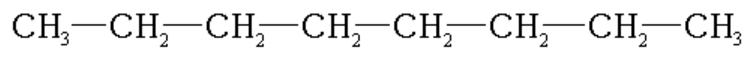
\includegraphics[width=350px]{Figures/bio/Prerequis/semi.png}
    \caption{\label{semi}Formule semi-développée de la molécule d'octane.}
  \end{center}
\end{figure}

Les atomes d'hydrogène étant présents partout, la représentation de molécules conséquentes devient rapidement lourde.
C'est dans le but de simplifier les représentations qu'à été inventée la formule semi-développée (voir figure \ref{semi}).
Les atomes d'hydrogène n'effectuant qu'une liaison 


\subsection{Représentation 1D d'une molécule : les SMILES}



\section{Graphes}